\clearpage
{\hspace{-5.5mm}\Huge Reading Guide}

The structure of this report is a variant of
\href{https://en.wikipedia.org/wiki/IMRAD}{IMRAD} adapted to engineering
projects. The structure follows the
\href{https://en.wikipedia.org/wiki/V-model}{V-model}, as shown in
\autoref{fig:v-model-report-structure}, extended with the academic parts:
\textit{Introduction}, \textit{Method}, \textit{Discussion} and
\textit{Conclusion}.

% ------------------------------------------------------------
% EXAMPLE of a DrawIO figure:
% The source file is assets/drawio/v-model.drawio - latexmk converts
% it to assets/drawio/v-model.pdf automatically before compiling.
% ------------------------------------------------------------
\begin{figure}[H]
  \centering
    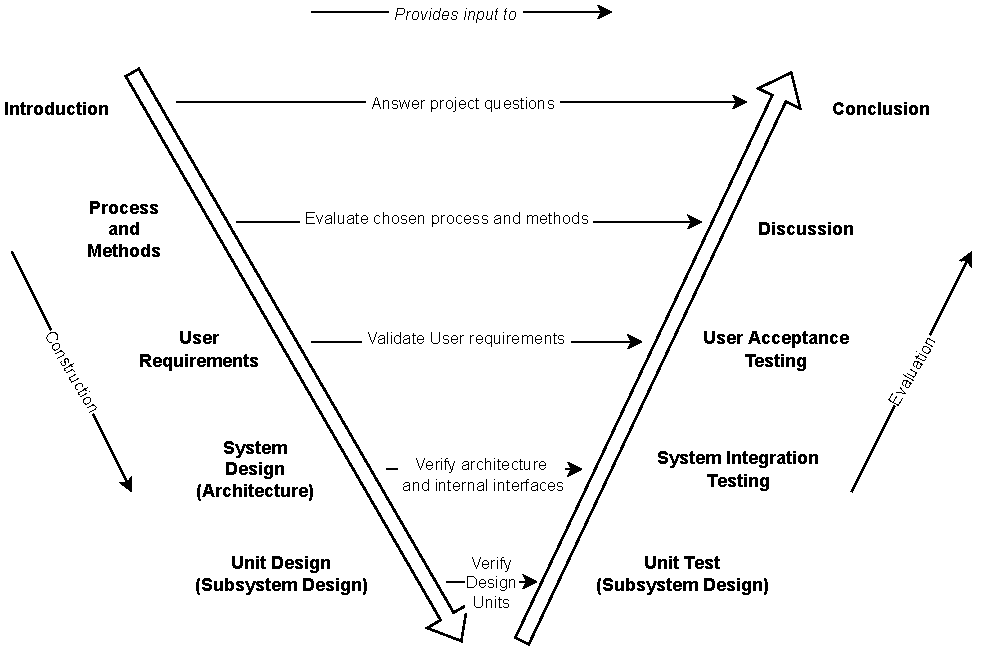
\includegraphics[width=\linewidth, trim=6cm 7.5cm 6cm 1.5cm, clip]{assets/drawio/v-model.pdf}
    \caption{Report structure based on the V-model}
    \label{fig:v-model-report-structure}
\end{figure}

In broad terms the report describes the project from idea, through
requirements, to architecture, design, test and evaluation.

